\section{Datasets}

\subsection{Obtaining a high-resolution dataset}
    
    
Super resolution is inherently a supervised learning task that needs the availability of HR data. In scenarios where HR data from sources like FOREST-2 is unavailable, an alternative is to generate synthetic images from external missions with characteristics similar to the FOREST-2 mission but with a superior spatial resolution.

\subsubsection{The ECOSTRESS mission}

NASA's ECOsystem Spaceborne Thermal Radiometer Experiment on Space Station (ECOSTRESS) mission is designed to provide new insights into the effects of the Earth's climate dynamics \cite{ECOSTRESS2023}, with a focus on the following scientific objectives:

\begin{enumerate}
    \item Identify the critical thresholds of water use and water stress in key climate-sensitive biomes, typically by observing the transition zones between biomes.
    \item Identify when plants stop consuming up water over the course of a day.
    \item Improve the accuracy of drought estimates based on agricultural water use in the continental United States. 
\end{enumerate}

ECOSTRESS employs thermal infra-red radiometers, specifically Prototype HyspIRI Thermal infra-red Radiometer \cite{PhyTIR2023} to measure the radiation emitted from the Earth's surface. It provides a spatial resolution of 69 meters with a temperature sensitivity of a few tenths of a degree \cite{ECOSTRESS2023}. The swath size is 400x400 km. The detector separates the energy from five different wavelengths using attached filters, producing five separate image layers for each scene. The pixels represent the intensity of thermal infra-red radiation emitted by the Earth's surface at each wavelength. The mission has a 4-day diurnal repeat cycle.

In the spatial domain, ECOSTRESS constitutes an excellent candidate for generating synthetic HR images, as its resolution constitutes approximately a threefold increase compared to FOREST-2. 

In the spectral domain, it is crucial to confirm the overlap between the mission bands. Given the narrower ECOSTRESS bands, the strategy will be averaging the radiances to align the spectral properties.
Fig. \ref{fig:5-wavelength-comparison} shows this spectral band comparison.
In the case of the LWIR1 FOREST band, the overlap is significant with the first three ECOSTRESS bands.
Although the overlap is less pronounced in the LWIR2 band, the radiation spectrum of black bodies at prevalent surface temperatures indicates the feasibility of constructing a synthetic LWIR2 from the last two ECOSTRESS bands. While FOREST's temporal resolution exceeds that of ECOSTRESS, allowing for the monitoring of new processes, this aspect is not the primary focus of the current study and will not be taken into account.



\begin{figure}[H]
    \centering
    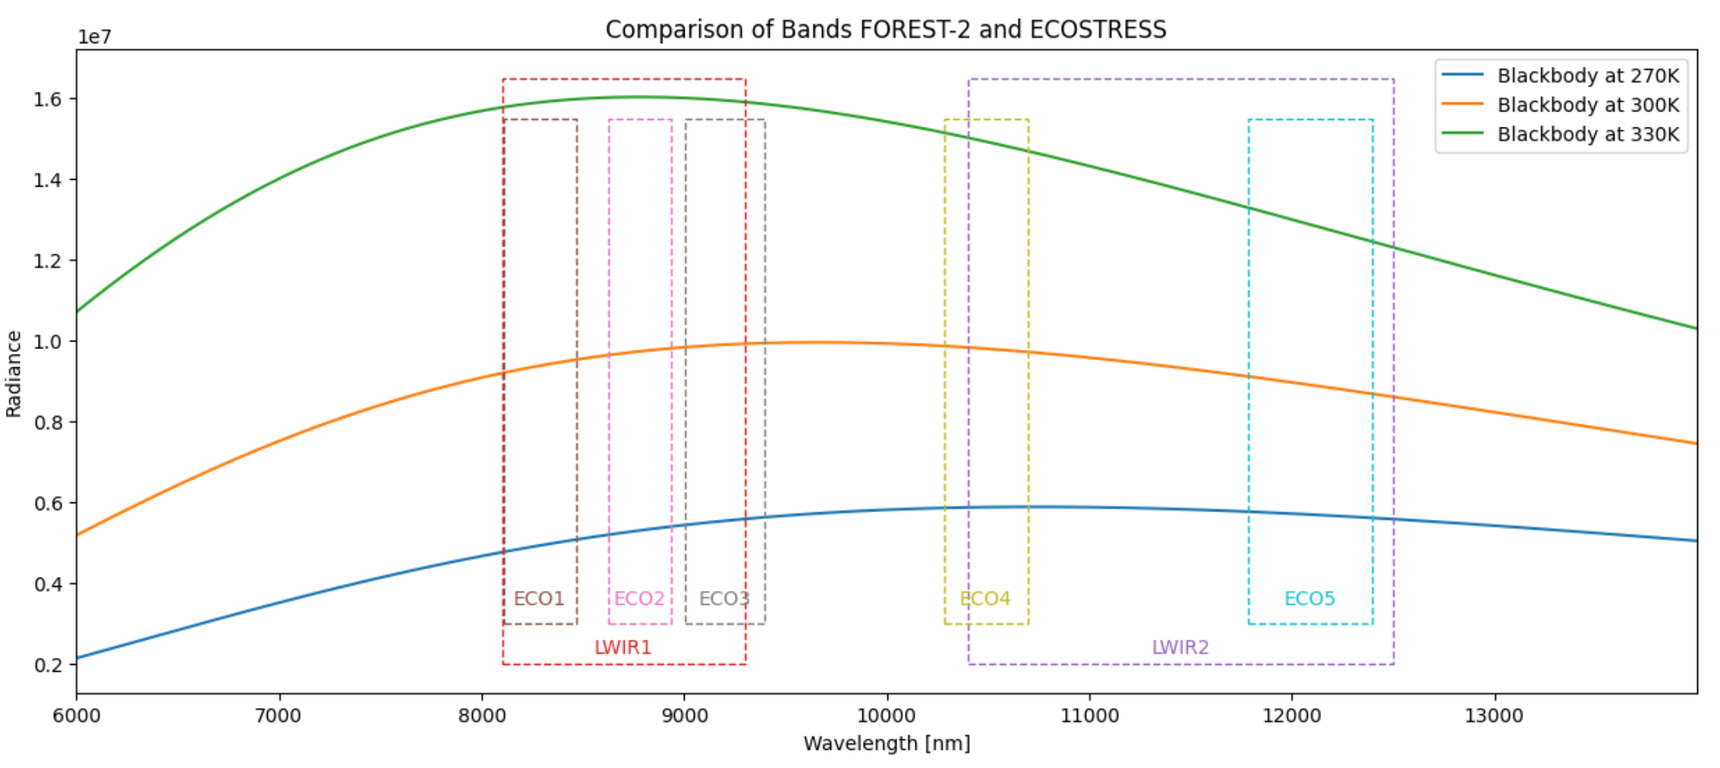
\includegraphics[width=\linewidth]{Includes/5-wavelength-comparison.png}
    \caption{Wavelengths of the sensors in ECOSTRESS and FOREST satellites. The radiation spectrum of black bodies at different temperatures is included for comparison.}
    \label{fig:5-wavelength-comparison}
\end{figure}

\subsubsection{ECOSTRESS scenes}
    ECOSTRESS imagery is available via NASA's Application for Extracting and Exploring Analysis Ready Samples (AppEEARS) \cite{AppEEARS2023}. This tool allows the request of area samples via vector polygons. Using the product's API \cite{AppEEARSAPI2023}, Level 1 Mapped Radiance scenes of size 200x200 km with center on the locations provided in Fig. \ref{fig:5-wavelength-comparison} were programmatically requested. Due to satellite hardware anomalies, certain spectral bands experienced acquisition gaps, needing a careful selection of date ranges to ensure the availability of all five bands \cite{ECO1BMAPRAD2023}.

   \begin{table}[h!]
        \centering
        \begin{tabular}{|l|l|}
        \hline
        Area     & 200 x 200 km                                                                              \\ \hline
        Products & \begin{tabular}[c]{@{}l@{}}Mapped Radiance (5 bands)\\ Quality (5 Bands)\end{tabular}     \\ \hline
        Dates    & \begin{tabular}[c]{@{}l@{}}2018/08/20 - 2019/03/04\\ 2023/05/01 - 2023/08/15\end{tabular} \\ \hline
        \end{tabular}
        \caption{Requests configuration}
        \label{tab:5-scenes-characteristics}
    \end{table}

    \begin{figure}[h!]
        \centering
        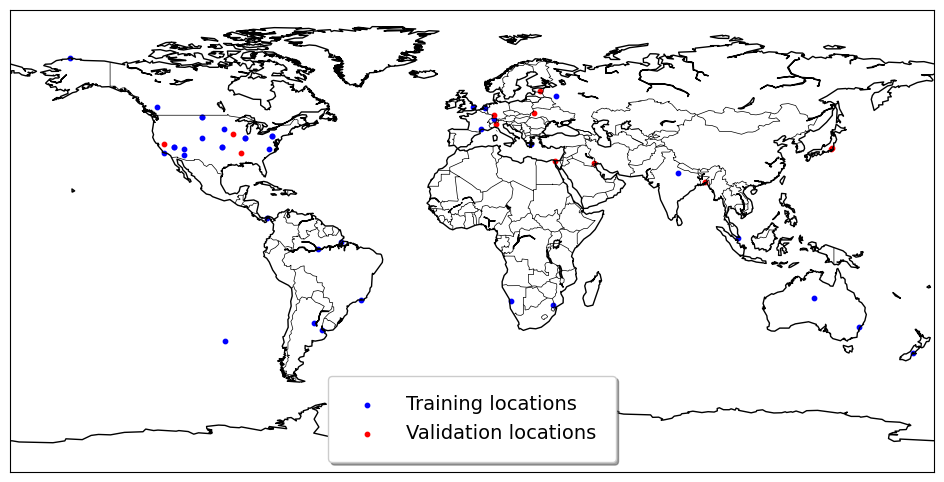
\includegraphics[width=\linewidth]{Includes/5-ecostress-map-location.png}
        \caption{Location of the samples taken from ecostress.}
        \label{fig:5-ecostress-map-location}
    \end{figure}

\subsubsection{Scene selection}

The AppEEARS platform returns multiple scenes that correspond to the specified area sample within the requested timeframe. This includes five mapped radiance measurements alongside their corresponding Quality Assurance (QA) bands. Additionally, a CSV file detailing quality statistics for each scene is provided. 

The interface returns any scene that overlaps with the requested area. For that reason, some GeoTIFFs from the same request area are significantly smaller than others, sometimes 90\% smaller. Moreover, an important number of these GeoTIFFs may contain a high percentage of bad-quality pixels, rendering them unsuitable for model training. Furthermore, as highlighted in the ECOSTRESS frequently asked questions \cite{ecostress_faq}, the accuracy of radiance measurements is highly dependent on clear sky conditions, as cloudy scenes typically yield negligible radiance emissions.

Downloading the entirety of the dataset is impractical due to its vast size.  
From the 50 requested areas, each one is potentially replicated over 20 times over the ten-month request window.
Such a dataset, given its magnitude, cannot be used for model training with the available hardware resources.
Therefore, a procedure is developed to identify and select the most appropriate scene for each month based on a predefined set of criteria:

\begin{enumerate}
\item Scenes should have a low proportion of bad-quality pixels.
\item Scenes should have a considerable size so that many crops can be taken from it.
\item As clouds imply low radiance values, clear sky scenes will have high radiance values.
\end{enumerate}


\begin{algorithm}[H] \label{alg:dataprocessing}
\caption{Process applied to the scenes returned from one area request.}
\begin{algorithmic}[1]

\State \textbf{QA statistics:}
\State Get the average proportion of good pixels $p_{gp}$ for the 5 radiances of the scene.
\State Discard scenes where $p_{gp} < 0.6 $ .

\State \textbf{Scene Statistics:}
\State Get the biggest scene of each month for each requested area.
\State Calculate the proportion between the size of each scene and the biggest of that month.
\State Discard images whose size proportion is smaller than 0.2.
\State Calculate the median of the radiance values of the scene.
\State \textbf{Selecting the scene of the month:}
\State Merge the QA statistics and the Scene statistics.
\State For each month, get the three scenes with the greatest $p_{gp}$.
\State Select the scene that has the greatest median radiance value.
\end{algorithmic}
\end{algorithm}

Applying this procedure, a dataset comprised of 5031 scenes taken from 50 area requests is reduced to 379 scenes.

\subsubsection{Data processing}

In order to be able to use the data in an SR model, a set of processing steps must be performed on it.
The diagram in Fig. \ref{fig:5-data_processing_flow_chart} displays the processing pipeline. The inputs are the 5 mapped radiance and their respective quality bands.
Mapped radiances 1,2 and 3 are averaged to form the HR LWIR1 synthetic FOREST-2, and mapped radiances 4 and 5 are averaged to form the HR LWIR2 synthetic FOREST-2. If any of the mapped radiances are missing, the corresponding HR image is discarded. 

The fill values in the mapped radiances and the data quality bands are used to create a binary mask for each spectral band. If a pixel is considered problematic, it is marked as a 1 in the binary mask. The QA band for an HR image is built using an OR operation on the corresponding mapped radiances involved in its construction. After being constructed, both the HR synthetic LWIR and the corresponding QA band are reprojected to the most suitable UTM EPSG code based on the latitude and longitude of the scene.

\begin{table}[H]
    \centering
    
    \label{tab:quality_classes}
    \begin{tabular}{cl}
        \toprule
        \textbf{Value} & \textbf{Description}                \\
        \midrule
        \multicolumn{2}{c}{Fill Value Classes}                \\
        -9997          & Pixel not seen                       \\
        -9998          & Missing data due to striping (not filled in) \\
        -9999          & Missing/bad data                     \\
        \midrule
        \multicolumn{2}{c}{Data Quality Classes}              \\
        0              & Good                                 \\
        1              & Missing stripe data, filled in       \\
        2              & Missing stripe data, not filled in   \\
        3              & Missing/bad data                     \\
        4              & Not seen                             \\
        \bottomrule
    \end{tabular}
    \caption{Fill Value and Data Quality Classes}
\end{table}

The synthetic LWIR images are not suitable for the super-resolution task yet.
They are too big to be kept in memory, and not all their values are of good quality.
For that reason, for each scene, a number of random crops of size 264x264 pixels are taken.
The random crop processor pipeline is displayed in Fig. \ref{fig:5-random_crop_processor}.
It is an iterative process where, at each stage, crops that do not comply with the quality considerations are discarded until the target number of crops per scene is achieved. Additionally, a translation operation is performed to the affine transformation of the geoTiff file, so that the crop can still be correctly georeferenced.


\begin{figure}[H]
    \centering
    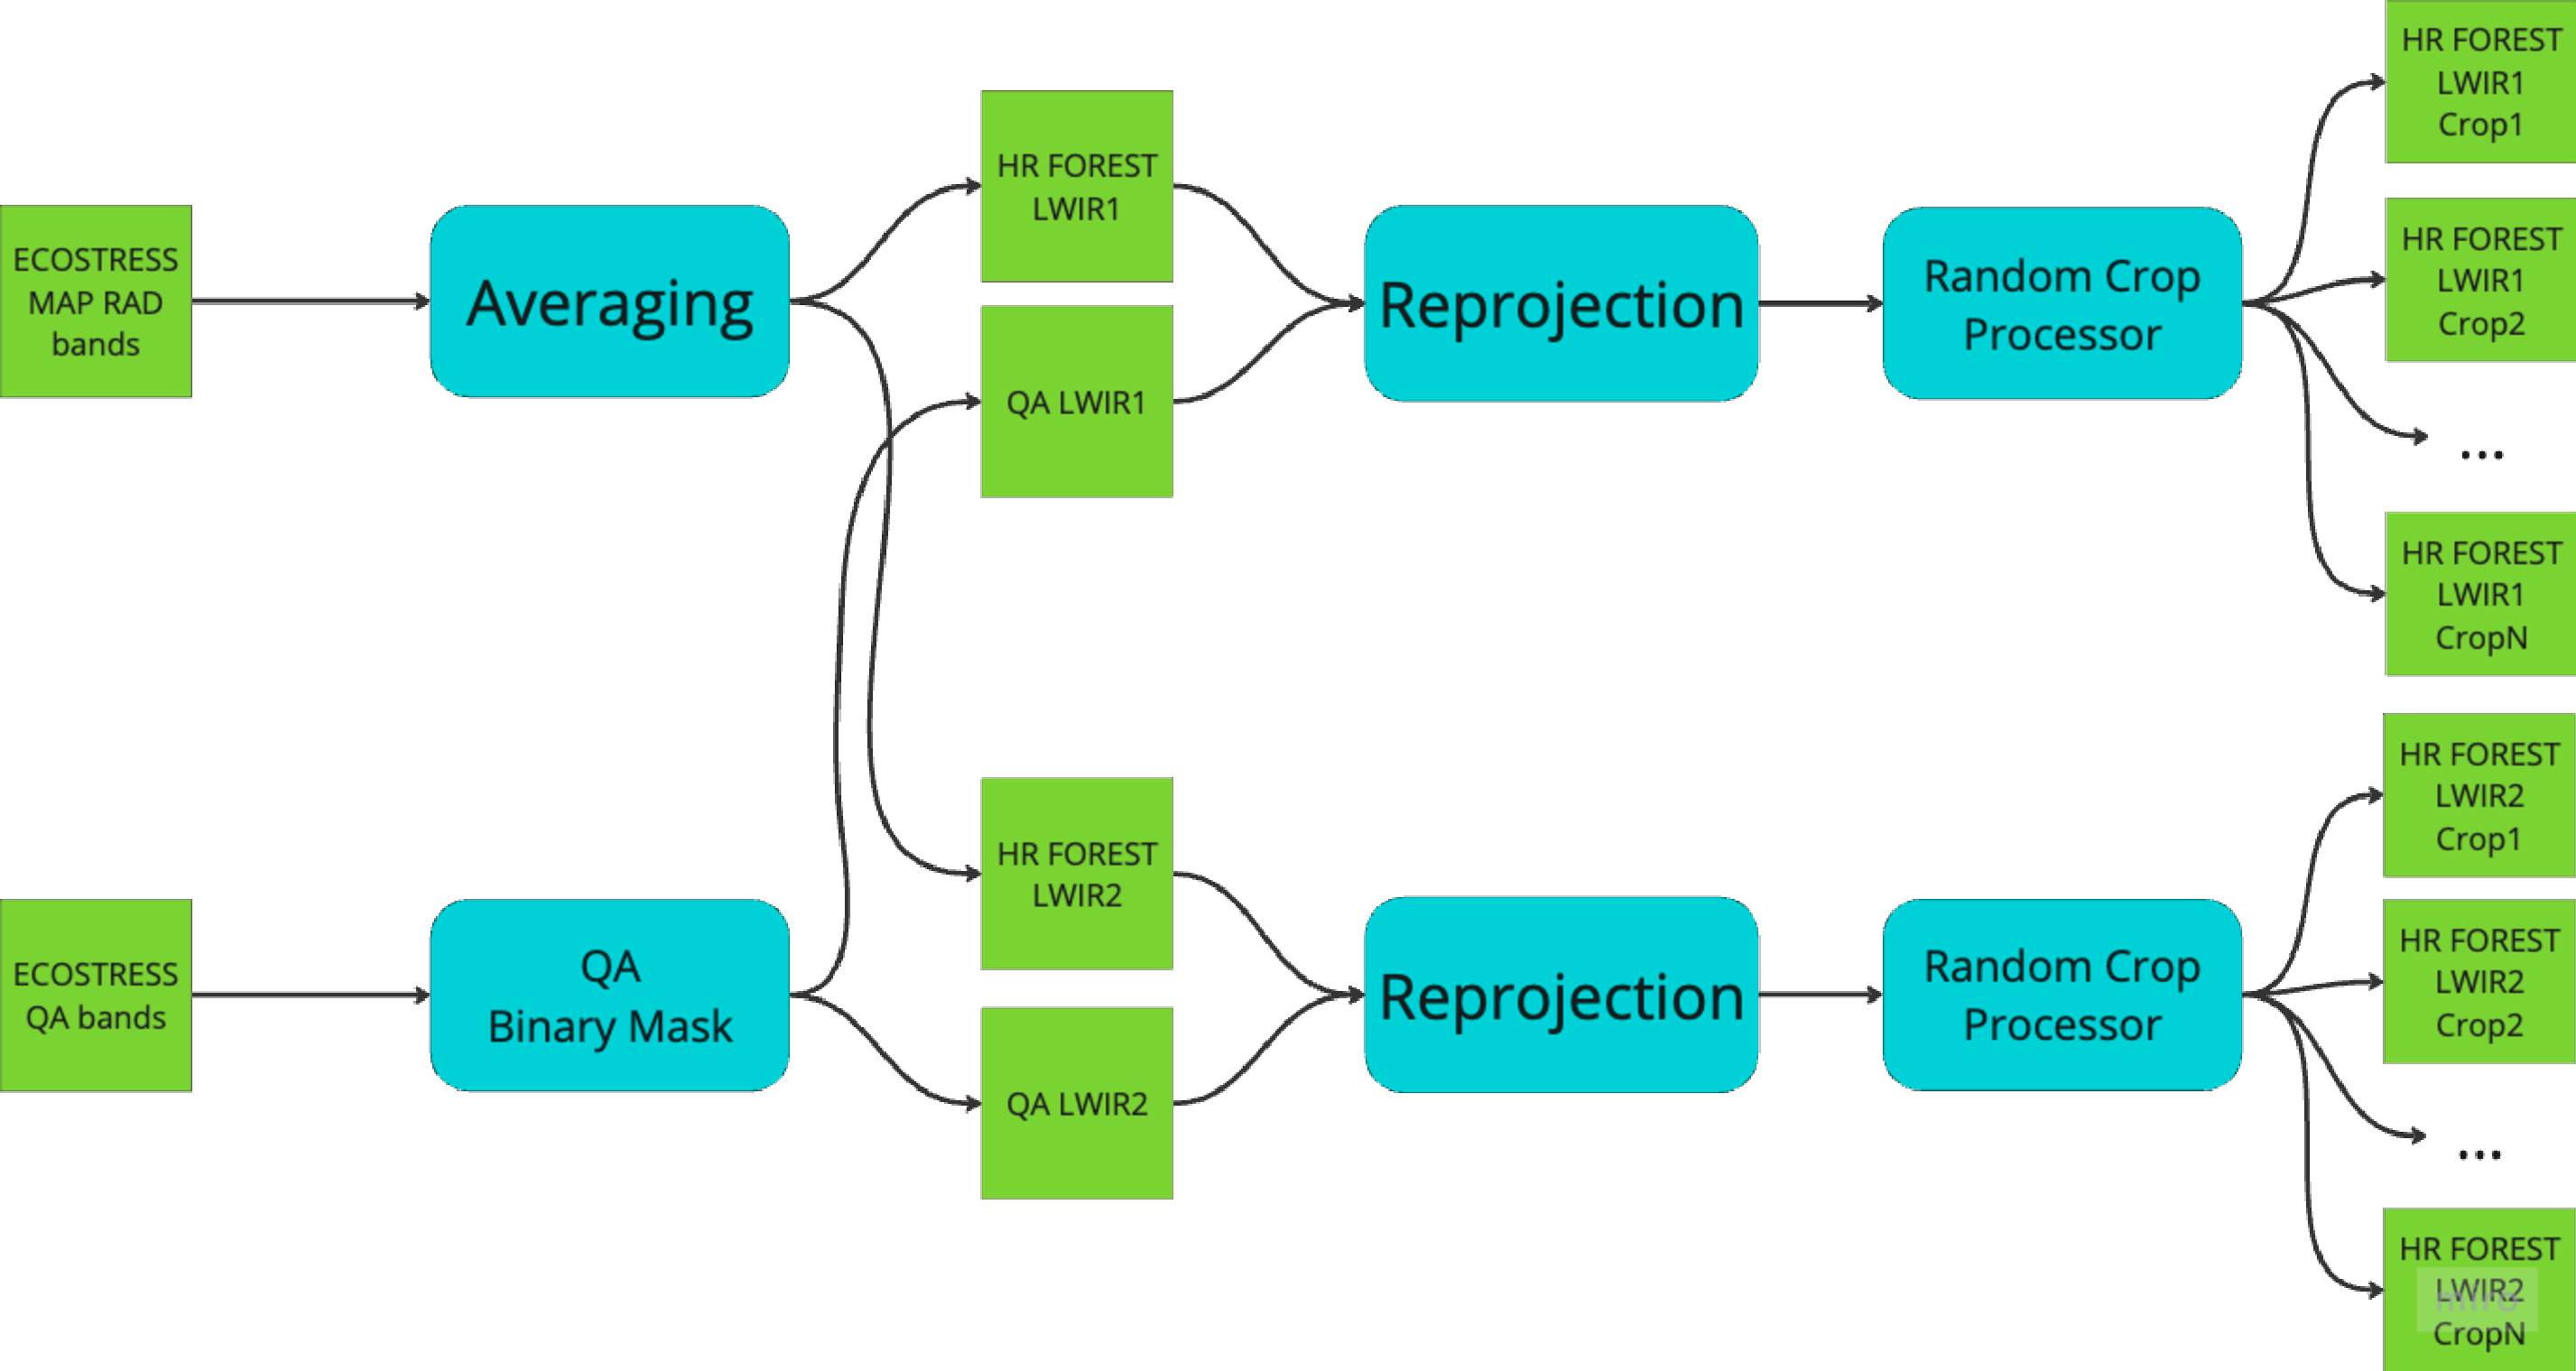
\includegraphics[width=\linewidth]{Includes/5-data_processing_flow_chart.pdf}
    \caption{Data processing workflow}
    \label{fig:5-data_processing_flow_chart}
\end{figure}

\begin{figure}[H]
    \centering
    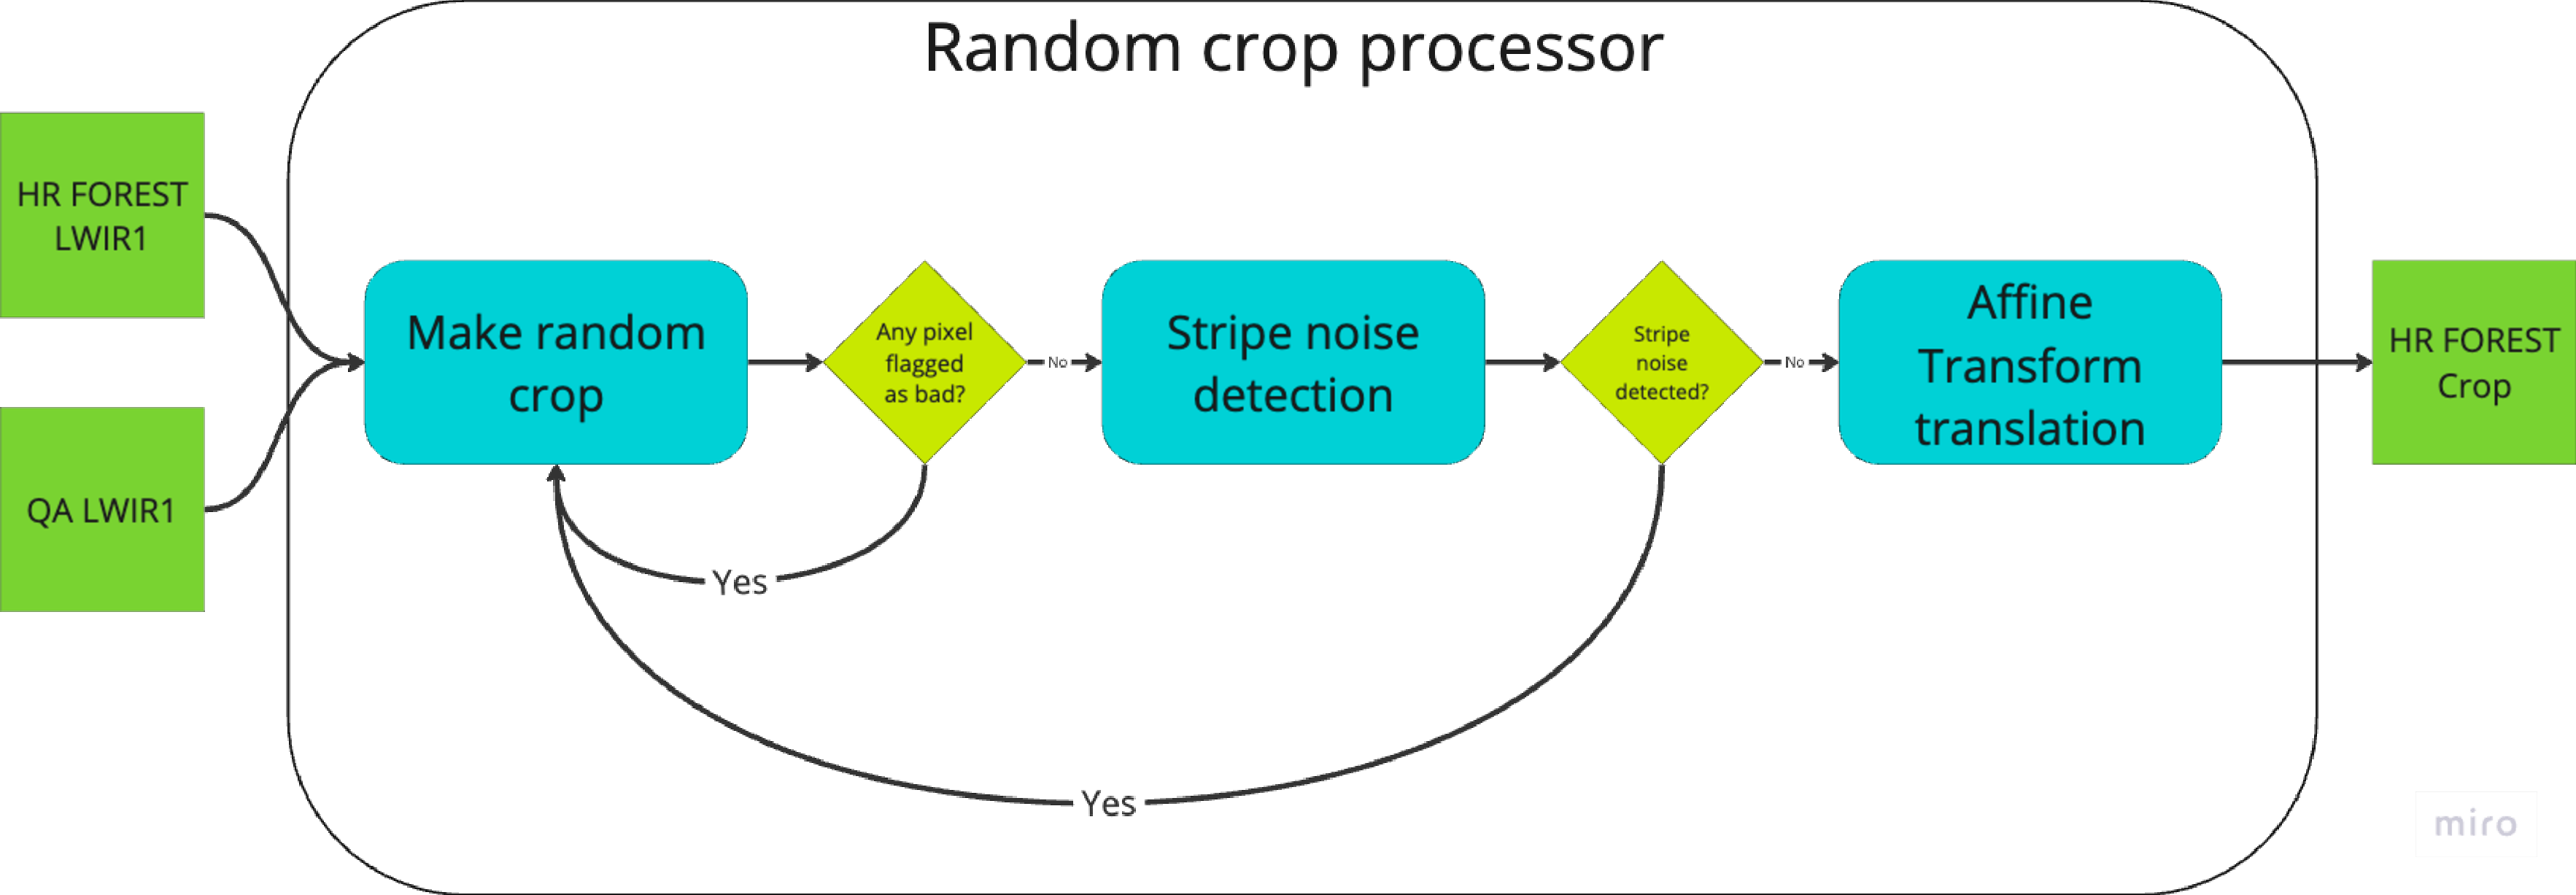
\includegraphics[width=\linewidth]{Includes/5-random_crop_processor.pdf}
    \caption{Random crop processor}
    \label{fig:5-random_crop_processor}
\end{figure}



\subsection{FOREST-2 scenes}

    To obtain a dataset of FOREST-2 images, the company provides an internal API that allows the download of scenes captured by the satellite. 
    The download of the scenes is done programmatically in the locations provided in Fig. \ref{fig:4-forest-locations}. 

    \begin{figure}[H]
        \centering
        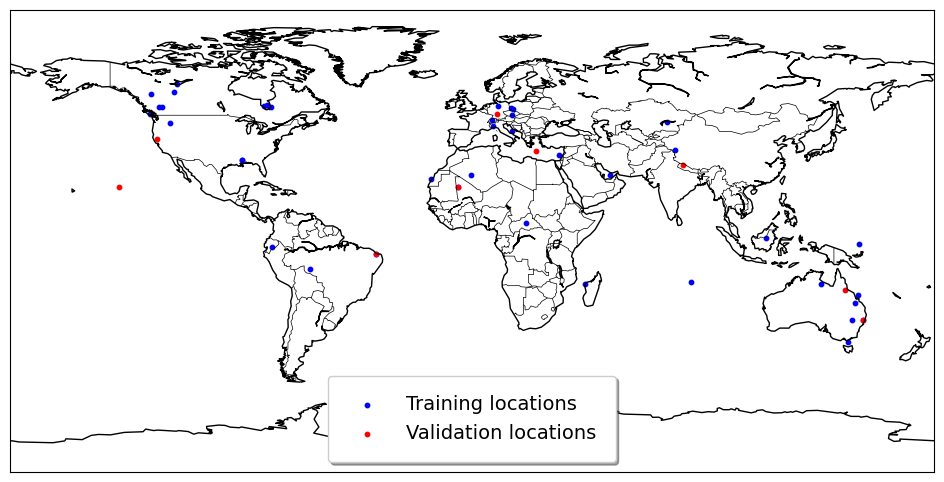
\includegraphics[width=\linewidth]{Includes/4-forest-locations.png}
        \caption{Location of the FOREST-2 scenes.}
        \label{fig:4-forest-locations}
    \end{figure}

    The scenes are downloaded in the NetCDF-4 format, containing the LWIR1, LWIR2, and MWIR bands, as well as the latitude and longitude information. 
    An example of a scene is shown in Fig. \ref{fig:4-forest-complete example}. 
    The focus of this work is on the long wave infra-red, which is the reason why the MWIR band is discarded.

    \begin{figure}[H]
        \centering
        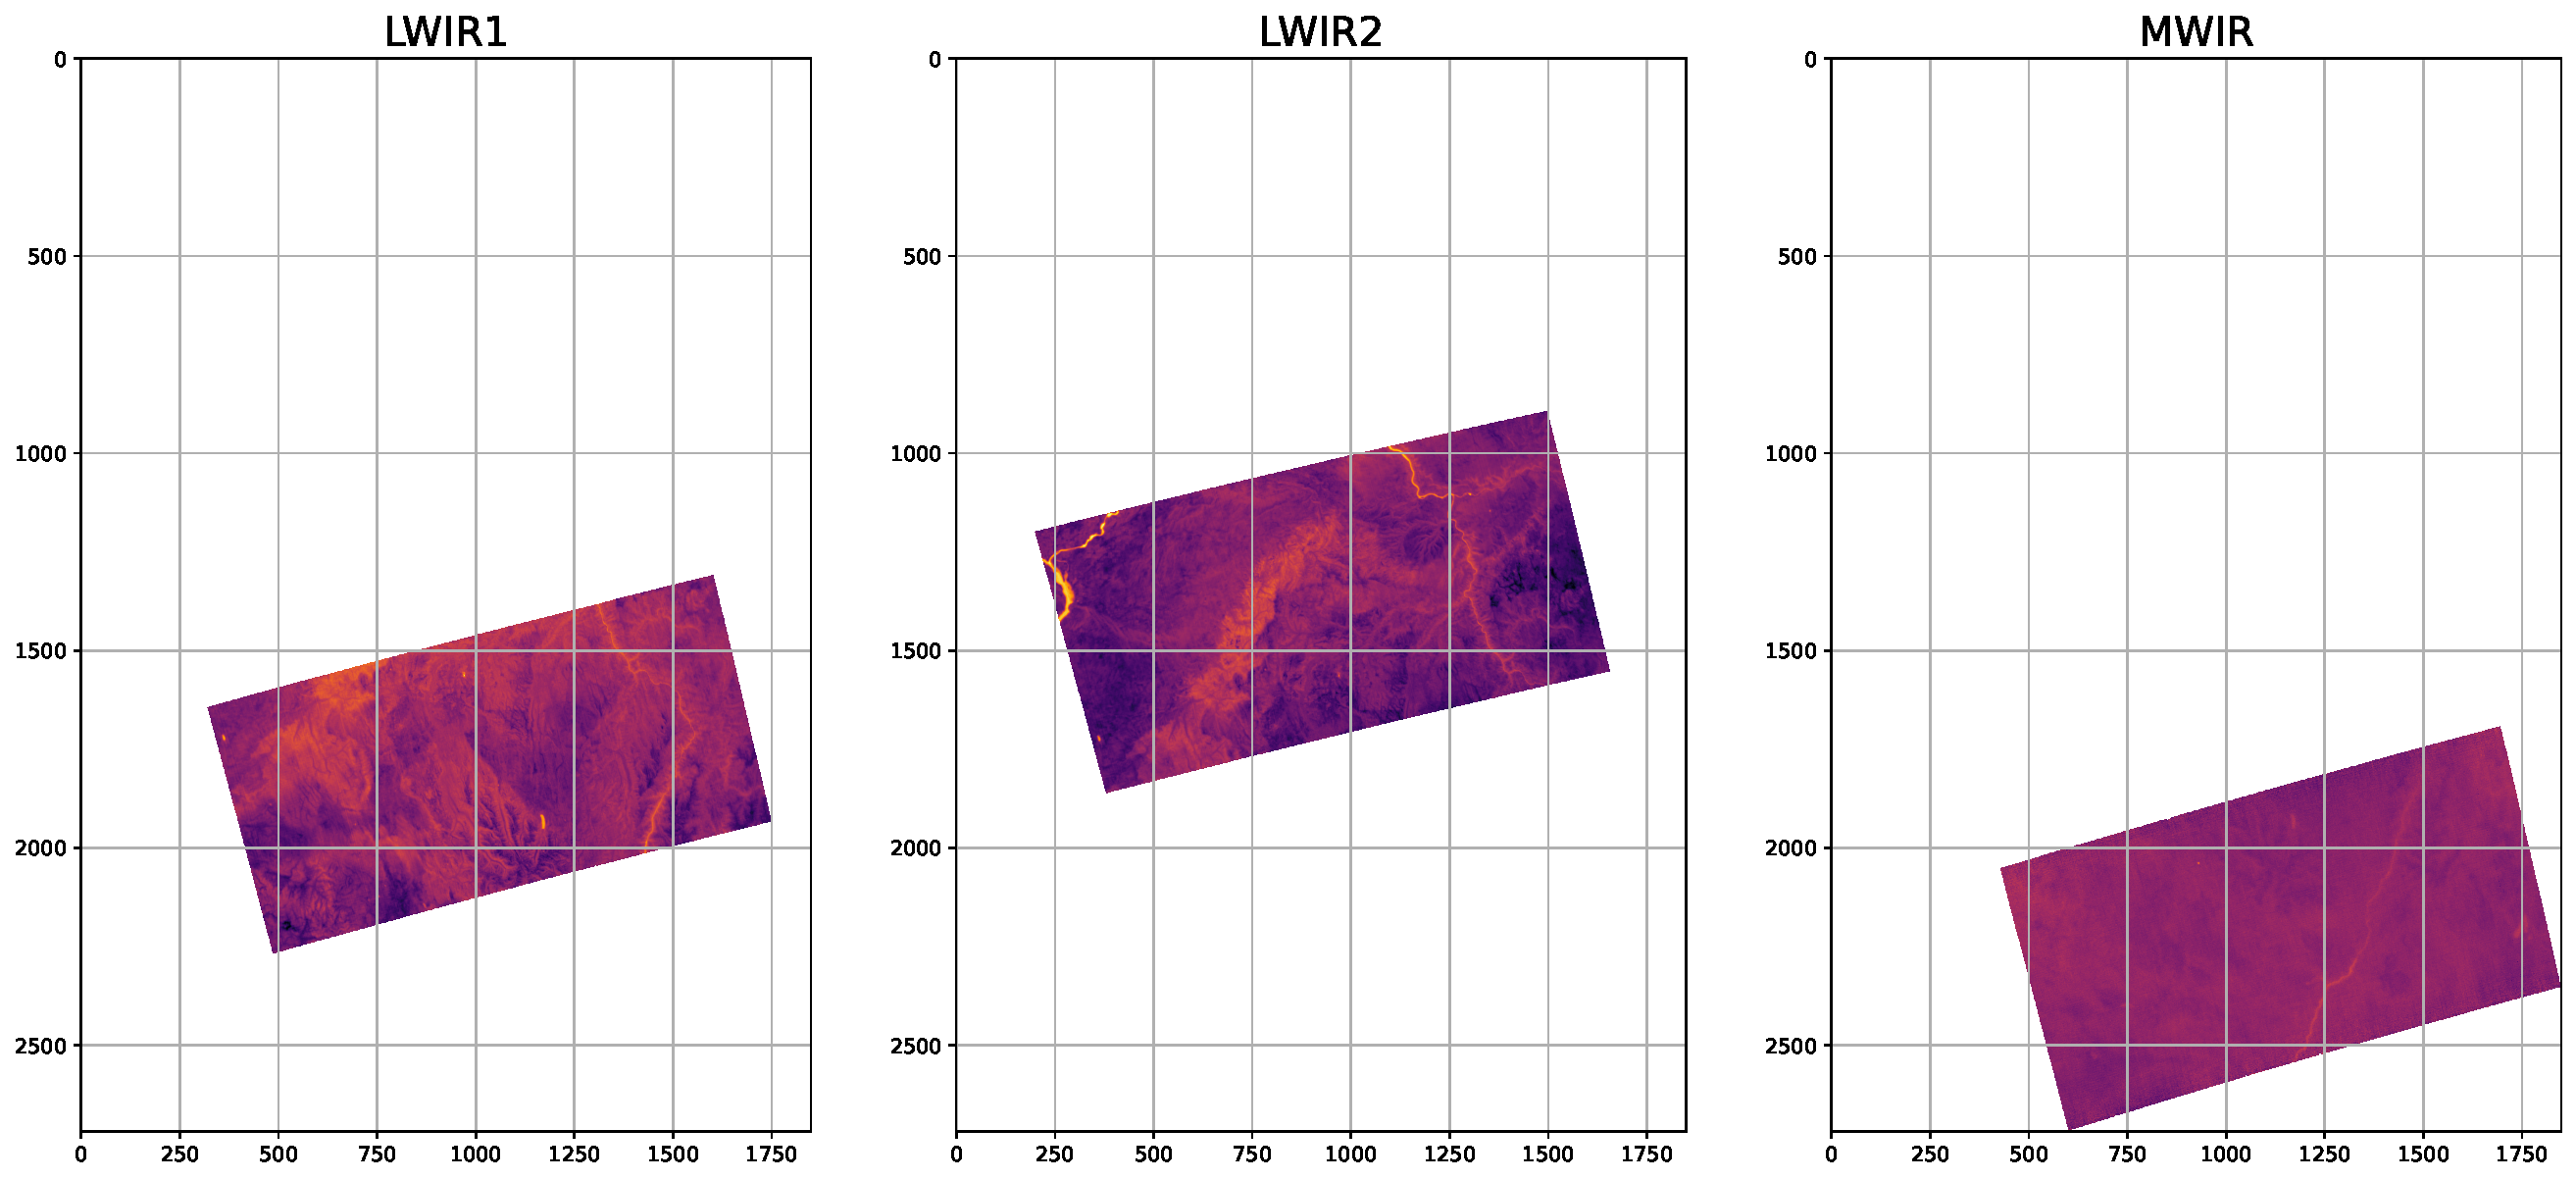
\includegraphics[width=\linewidth]{Includes/4-forest2-unprocessed-bands.pdf}
        \caption{LWIR1, LWIR2, and MWIR bands of a FOREST-2 scene downloaded using the company's API.}
        \label{fig:4-forest-complete example}
    \end{figure}

    \subsubsection{Data processing}

    The provided arrays have an enormous proportion of NA values and are not suitable for taking crops.
    For that, a bounding box is defined for each band, removing most of the NA values. 
    The resulting scenes are shown in Fig. \ref{fig:4-forest-bounding-box}.

    \begin{figure}[H]
        \centering
        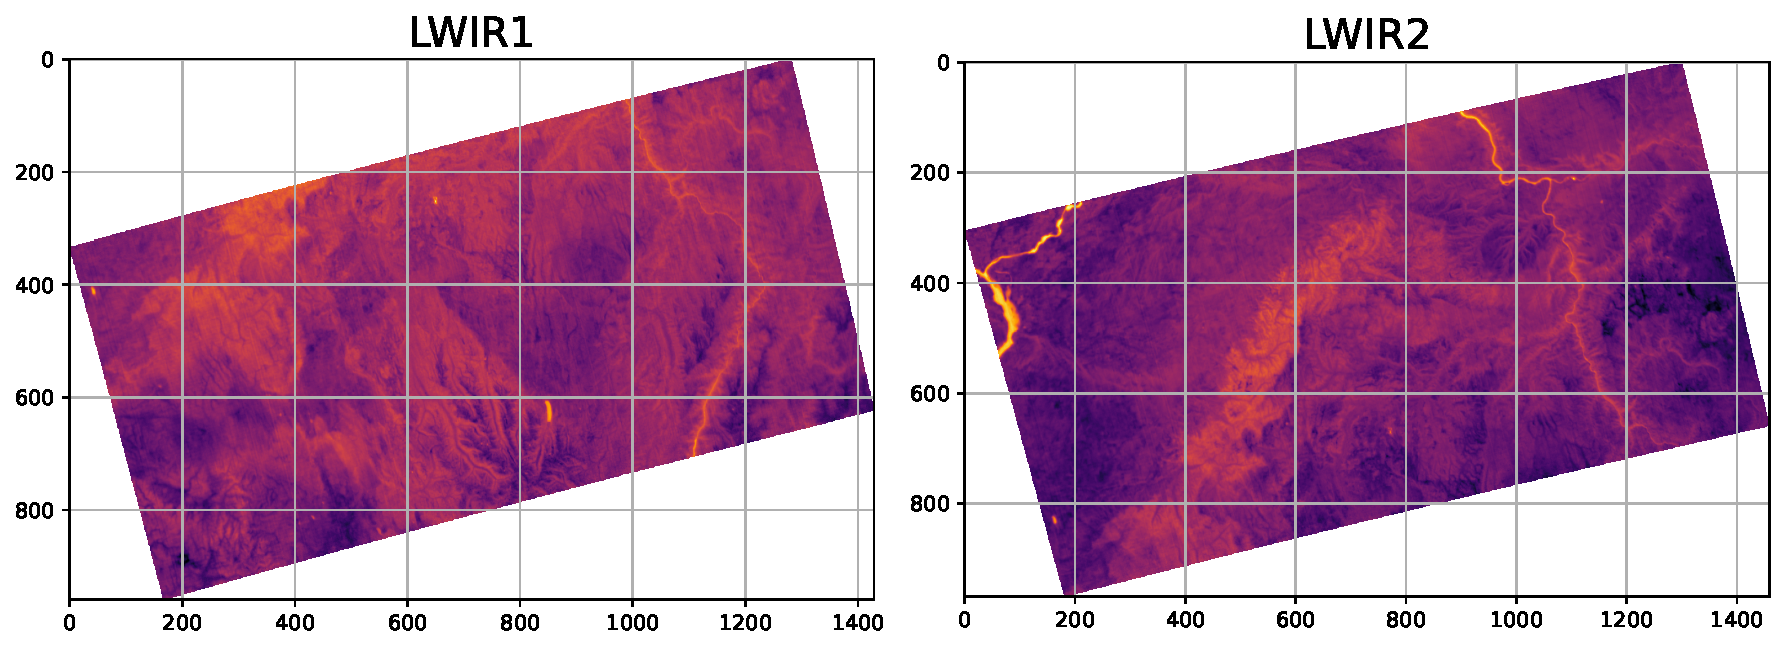
\includegraphics[width=\linewidth]{Includes/4-forest2-cropped-bands.pdf}
        \caption{LWIR1 and LWIR2 of a FOREST-2 scene downloaded using the company's API, after cropping NA values.}
        \label{fig:4-forest-bounding-box}
    \end{figure}

    A similar random crop processor as in Fig. \ref{fig:5-random_crop_processor} is used afterward. 
    The objective is to obtain several crops of size 88x88 pixels that match the 264x264 pixels of the synthetic HR FOREST-2 images when upscaled by a factor of 3.
    If a crop has  NA values or stripe noise is detected, it is discarded and the process restarts, with a maximum of one hundred retries.
    Using the latitude and the longitude information, the affine transformation is calculated so that the crops can be georeferenced, if necessary.
    
\subsection{Datasets}

The implemented Pytorch dataset class loads and yields samples from two different file locations, one for the HR images (source domain) and another for the LR images (target domain). 
The source domain consists of synthetic HR FOREST-2 images produced from ECOSTRESS. The target domain is composed of LR images which can be either artificially degraded, or real FOREST-2 LR images.
The samples are usually unpaired, meaning that the scenes are not compared on an image-to-image basis. Still, the implementation allows the use of paired datasets in order to calculate supervised metrics. 
In the case a domain has less samples than another, the class will bootstrap it so the sizes match.

\begin{table}[H]
    \centering
    \resizebox{\textwidth}{!}{%
    \begin{tabular}{|c|cccc|cccc|}
    \hline
                & \multicolumn{4}{c|}{$\mathcal{D}_{\text{SF}-\text{SF}}$}                                                                                                                                                                                                                                         & \multicolumn{4}{c|}{$\mathcal{D}_{\text{SF}-\text{RF}}$}                                                                                                                                                                                                               \\
                & \multicolumn{2}{c|}{Training}                                                                                                                             & \multicolumn{2}{c|}{Validation}                                                                                                      & \multicolumn{2}{c|}{Training}                                                                                                                & \multicolumn{2}{c|}{Validation}                                                                                         \\ \hline
    Domain      & Source                                                       & \multicolumn{1}{c|}{Target}                                                                & Source                                                       & Target                                                                & Source                                                       & \multicolumn{1}{c|}{Target}                                                   & Source                                                       & Target                                                   \\ \hline
    Image type      & \begin{tabular}[c]{@{}c@{}}Synth HR \\ FOREST-2\end{tabular} & \multicolumn{1}{c|}{\begin{tabular}[c]{@{}c@{}}Degraded Synth \\ HR FOREST-2\end{tabular}} & \begin{tabular}[c]{@{}c@{}}Synth HR \\ FOREST-2\end{tabular} & \begin{tabular}[c]{@{}c@{}}Degraded Synth\\  HR FOREST-2\end{tabular} & \begin{tabular}[c]{@{}c@{}}Synth HR\\  FOREST-2\end{tabular} & \multicolumn{1}{c|}{\begin{tabular}[c]{@{}c@{}}Real \\ FOREST-2\end{tabular}} & \begin{tabular}[c]{@{}c@{}}Synth HR\\  FOREST-2\end{tabular} & \begin{tabular}[c]{@{}c@{}}Real\\  FOREST-2\end{tabular} \\ \hline
    Crop number & 13764                                                        & \multicolumn{1}{c|}{13764}                                                                 & 2676                                                         & 2676                                                                  & 13764                                                        & \multicolumn{1}{c|}{4000}                                                     & 2676                                                         & 1200                                                     \\ \hline
    Crop size   & 264                                                          & \multicolumn{1}{c|}{88}                                                                    & 264                                                          & 88                                                                    & 264                                                          & \multicolumn{1}{c|}{88}                                                       & 792                                                          & 264                                                      \\ \hline
    Scale ratio & 3                                                            & \multicolumn{1}{c|}{3}                                                                     & 3                                                            & 3                                                                     & 3                                                            & \multicolumn{1}{c|}{3}                                                        & 3                                                            & 3                                                        \\ \hline
    Paired?     & \multicolumn{2}{c|}{No}                                                                                                                                   & \multicolumn{2}{c|}{Yes}                                                                                                             & \multicolumn{2}{c|}{No}                                                                                                                      & \multicolumn{2}{c|}{No}                                                                                                 \\ \hline
    \end{tabular}%
    }
    \caption{Dataset characteristics}
    \label{tab:dataset_characteristics}
    \end{table}


\subsubsection{Synthetic FOREST-2 - degraded synthetic FOREST-2}
    The dataset $\mathcal{D}_{\text{SF}-\text{SF}}$ is built by taking the HR synthetic FOREST-2 crops and applying the baseline degradation model proposed in \ref{subsec:baseline_degradation_model}. 
    The 264x264 crops are reduced to 88x88. The training set is used to train the SR model, while the validation set is used to monitor the training process and avoid overfitting. 
    Even though, in this case, the HR and LR versions of the same scene are available, the training dataset is unpaired by shuffling the samples.
    The validation set is not shuffled, and thus, metrics like PSNR and SSIM can be calculated in the target domain. The parameters used for the degradation model are described below:

    \begin{table}[H]
        \centering
        \begin{tabular}{l|l}
        Parameter & Value \\ \hline
        downscaling ratio & 3 \\ 
        Gaussian Kernel size & 21 \\ 
        Gaussian kernel sigma in X axis &  $\sim \mathcal{N}(1,0.3)$  \\ 
        Gaussian kernel sigma in Y axis &  $\sim \mathcal{N}(1,0.3)$  \\ 
        target radiometric error & 1.5K \\ 
        white noise factor & 0.5 \\ 
        constant noise factor & 0.5 \\ 
        \end{tabular}
        \caption{Parameters used in the degradation model employed to generate the $\mathcal{D}_{\text{SF}-\text{SF}}$ dataset.}
        \label{tab:degradation_model_parameters}
    \end{table}

\subsubsection{Synthetic FOREST-2 - real FOREST-2}
    The dataset $\mathcal{D}_{\text{SF}-\text{RF}}$ is composed of the 264x264 synthetic HR FOREST-2 crops as the source domain and  88x88 real FOREST-2 crops as the target domain. 
    The validation dataset is not paired, as the HR and LR images are entirely different scenes.
    Thus, supervised metrics are not available for the super-resolved target domain images. 
    The metric used to determine the best model is the PSNR from the super resolution of the output of the degradation model generator.

\subsubsection{Paired data acquisition} \label{subsec:pairedacquisition}

    When two missions pass over the same geographic region in a relatively similar timeframe, the overlap between their recorded scenes allows the collection of paired datasets. In order to do this with ECOSTRESS and FOREST-2, the trajectory of both missions is closely monitored to detect when they are close enough for data acquisition. As the intersection of the trajectories is not a perfect match, some processing must be done to co-register the images taken from both satellites. 

    In the case of ECOSTRESS and FOREST-2, paired data would be available once per week. However, because of issues in data quality from both missions or atmospheric factors such as cloud cover, only a single scene was successfully captured in the timeframe of this work. Although the amount of images is not sufficient to create a proper validation dataset, the scene will be used to assess the performance of the SR models. To avoid errors on the PSNR due to wrong co-registration of the images, the adjusted metrics explained in \ref{subsec:adjustedmetrics} will be used.




\newpage